\section{Artificial density bumps}\label{density_bump}
We first consider discs initialised with a density bump. Our aim here
is to examine the effect of (layered) viscosity on the RWI
\emph{through the linear perturbation}, assuming a density bump can be
formed in the first place.  

We therefore require the initial conditions to be that of a steady
state disc with a density bump in the presence of viscosity. This
permits us to define a linear instability in the usual way 
(i.e. perturbations are measured with respect to a steady
equilibrium). We do this by choosing the initial cylindrical radial
velocity $v_{Ri}$ and viscosity profile appropriately, as described
below. 

\subsection{Initial cylindrical radial velocity}
For axisymmetric flow with angular velocity that only depends on the
cylindrical radius, the azimuthal momentum equation reads 
\begin{align}\label{ang_mom_cons}
  R\rho v_R\frac{\p}{\p R}\left(R^2\Omega \right) = \frac{\p}{\p
    R}\left(R^3\rho\nu\frac{\p\Omega}{\p R}\right). 
\end{align}
Assuming a steady state with $v_z=0$, mass
conservation (Eq. \ref{cont_eq}) implies that the mass flux  
$\dot{M}\equiv R\rho v_R$ is independent of $R$. In this case,
Eq. \ref{ang_mom_cons} can 
be integrated once to yield 
\begin{align}\label{temp}
  \dot{M}R^2\Omega = R^3\rho\nu\Omega^\prime + C(z) \quad \text{if $\p_R\dot{M}$} = 0, 
\end{align}
where $^\prime$ denotes $d/dR$ and $C(z)$ is an arbitrary function of
$z$. Eq. \ref{temp} motivates the simple choice
\begin{align}\label{init_vr} 
  v_{Ri} = \frac{\nu}{R}\frac{d\ln{\Omega_i}}{d\ln{R}} 
\end{align}
for the initial cylindrical radial velocity. Next, we choose the
viscosity profile $\nu$ to make the mass flux independent of
cylindrical radius.  

\subsection{Viscosity profile for a steady state}\label{visc_model}
If the initial disc corresponds to a steady state, then
$R \rho_i v_{Ri}$ can only be a function of $z$. With $v_{Ri}$ chosen by Eq. \ref{init_vr}, this implies
$R\rho_i\nu\Omega_i^\prime/\Omega_i$ is only a function of $z$. We are
therefore free to choose the vertical dependence of viscosity.  

Let $\nu = \hat{\nu}r_0^2\Omega_K(r_0)$, where
$\hat{\nu}=\hat{\nu}(R,z)$ is a dimensionless function describing
the magnitude and spatial distribution of the axisymmetric kinetmatic
viscosity. We choose $\hat{\nu}$ such that   
\begin{align}\label{visc_profile}
  \hat{\nu}\rho_i(R,z)\frac{d\ln{\Omega_i}}{d\ln{R}} =
  \hat{\nu}_0\left[1+Q(z/H_0)\right]\rho_i(r_0,z)\left.\frac{d\ln{\Omega_i}}{d\ln{R}}\right|_{r_0}, 
\end{align}
where $\nu_0$ is a constant dimensionless floor viscosity and   
\begin{align}\label{step}
  Q(\zeta) = \frac{\left(A_\nu - 1\right)}{2}
  \left[  2 + \tanh{\left(\frac{\zeta - \zeta_\nu}{\Delta\zeta_\nu}\right)}
    %  \left. 
    - \tanh{\left(\frac{\zeta +
        \zeta_\nu}{\Delta\zeta_\nu}\right)}\right]
\end{align}
is a generic function describing a step of magnitude
$A_\nu-1$. The position and width of the step is described by
$\zeta_\nu$ and $\Delta\zeta_\nu$, respectively. 
In Eq. \ref{visc_profile} we have set the dimensionless co-ordinate
$\zeta=z/H_0$ where $H_0=H(r_0)$.  

Eq. \ref{visc_profile} implies that at the fixed cylindrical radius
$R=r_0$, the dimensionless viscosity increases from $\hat{\nu} =
\hat{\nu}_0$ at the midplane to $\hat{\nu} = A_\nu\hat{\nu}_0$ for
$z > \zeta_\nu H_0$. An example of such a layered viscosity profile
profile is depicted in Fig. \ref{visc2d}. 

\begin{figure}
  \centering
  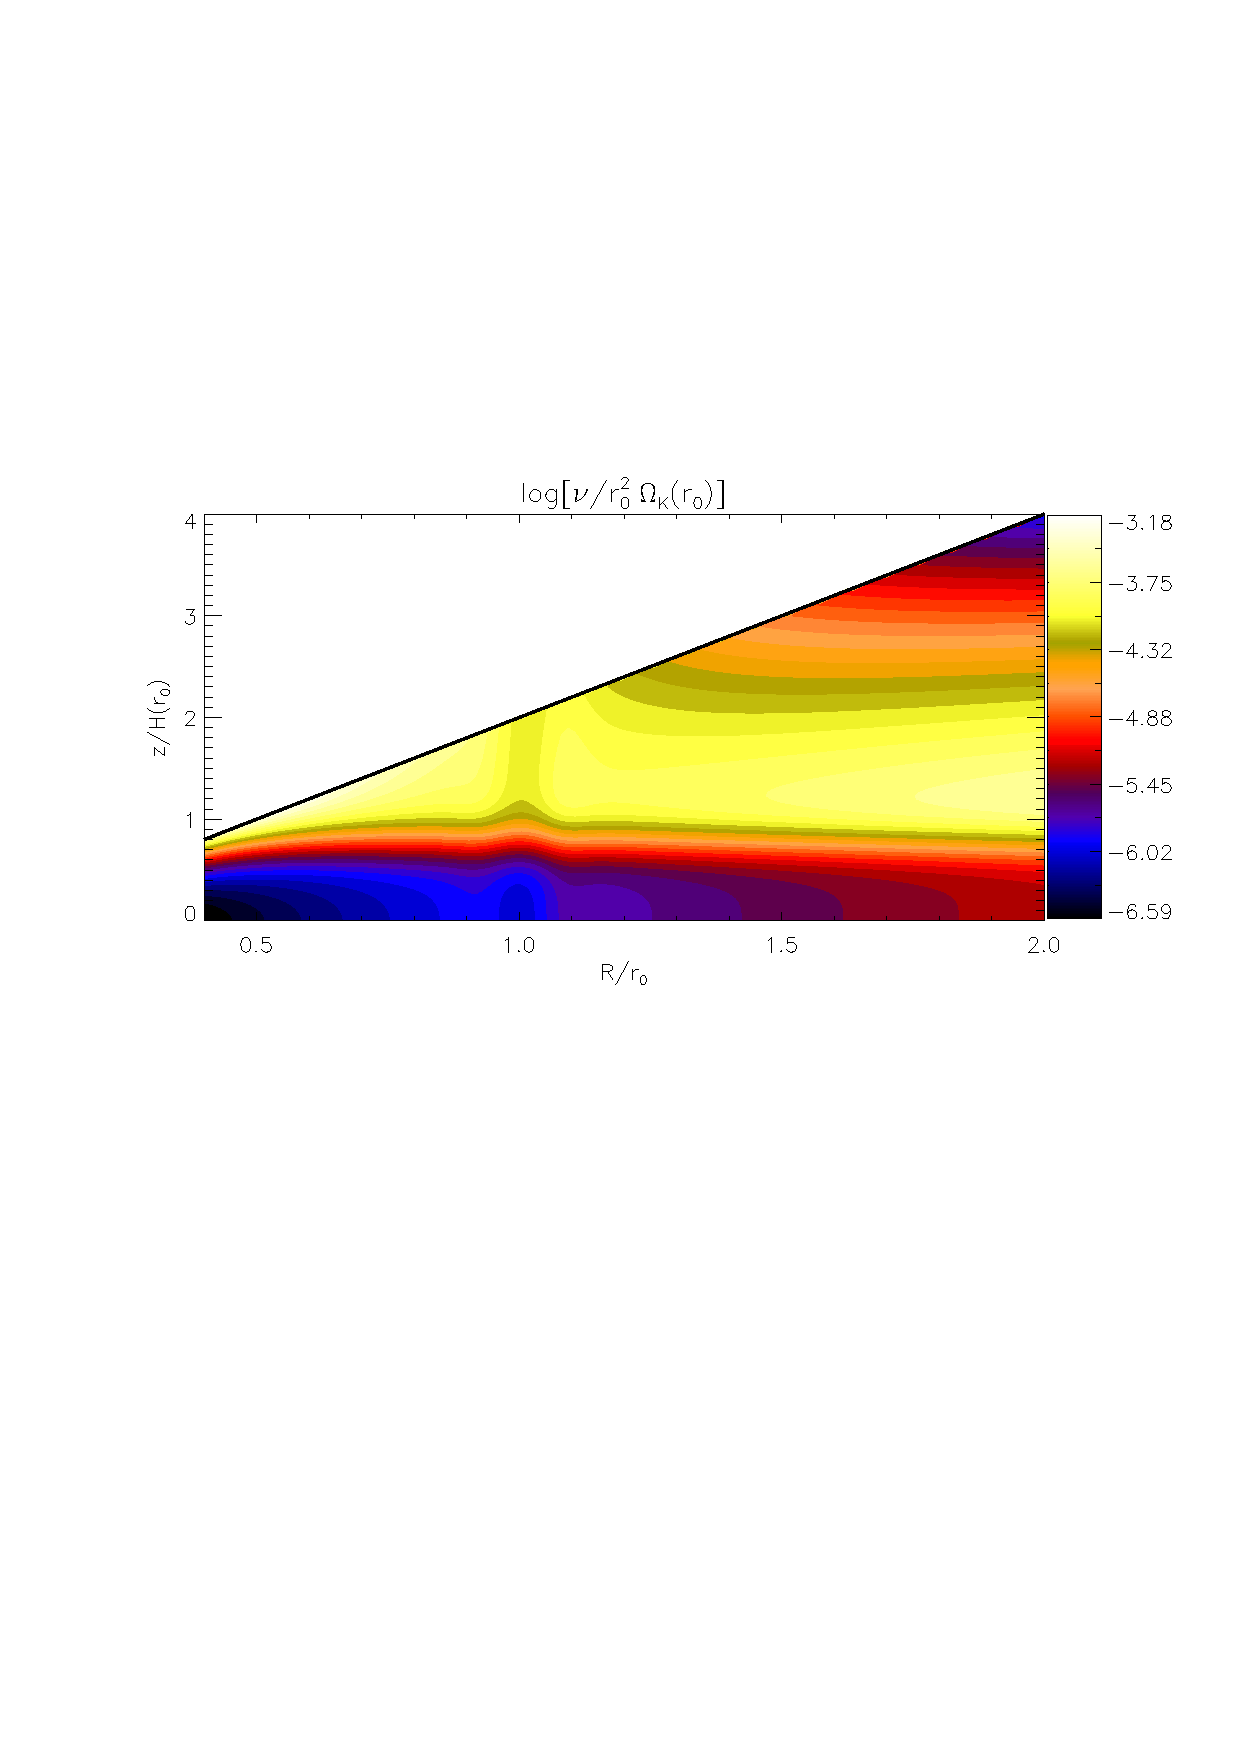
\includegraphics[width=\linewidth]{figures/pdisk_visc2d_layer2}
  \caption{Example of a two-layered kinematic viscosity profile
    resulting from Eq. \ref{visc_profile}. This specific plot
    corresponds to case V2. The solid line
    delineates the upper boundary of the computational domain.
    \label{visc2d}}
\end{figure}

\subsection{Simulations}
We consider discs with radial extent $[\rin,\rout]=[0.4,2.0]r_0$,
vertical extent with $n_h=2$ scale-heights and aspect-ratio $h=0.1$ at
$R=r_0$. We use $(N_r, N_\theta,
N_\phi)=(256,64,512)$ grid points. 
The resolution at the reference radius is then
$16,\,32,\,8$ cells per scale-height in $r,\theta,\phi$ directions,
respectively. The planetary potential is disabled for these runs
($M_p\equiv 0$).    

The bump parameters are set to $A=1.25$ and $\Delta R = 0.05r_0$ for
all runs in this section. The spherical radial velocity is subject 
to random perturbations of magnitude 
$10^{-4}c_s$ a few time-steps after initialisation. 

\subsubsection{Inviscid run}
For reference we simulate an effectively inviscid disc, case B0,
with the viscosity parameters $\hat{\nu}_0=10^{-9}$ and $A_\nu = 1$.  
The latter implies the viscosity is independent of $z$ at $R=r_0$.   

%% Two simulations were run for with setup. Case B0 with a
%% reflective upper boundary and case B1 with an unperturbed upper
%% boundary. 

Inviscid setups similar to case B0 have previously been simulated
both in the linear and nonlinear regimes  \citep{meheut12, lin13}. So,
in addition to a control run, case B0 also serves to test the \pluto
code in simulating the RWI.    

\subsubsection{Viscous runs}
In these runs the floor viscosity is fixed to
$\hat{\nu}_0=10^{-6}$. The control run  case V0 with $A_\nu =
1$. Thus, case V0 is the viscous version of case B0.  

We then consider models where the kinematic viscosity increases by
a factor $A_\nu=100$ for $z>\zeta_\nu H_0$ at the bump radius. We
choose $\zeta_\nu=1.5,\,1.0$ for cases V1 and V2, respecively.  This gives a upper 
viscous layer of thickness $0.5H$ and $H$ at $R=r_0$. (See
Fig. \ref{visc2d} for a plot of the kinematic viscosity profile for case V2.) 
For case V1 and V2 the transition thickness is fixed to
$\Delta\zeta_\nu=0.2$.  
 
Finally, we consider a high viscosity run, case V3, with $\zeta_\nu =
0$, i.e. the viscous layer occupies the entire vertical domain. Note
that this is equivalent to setting $\hat{\nu}_0=10^{-4}$ and $A_\nu=1$. 

\subsection{Results}
Table \ref{artificial_bump} summarises the simulations presented in
this section, along with several diagnostic measures 
of each case.  
The linear mode growth rates are measured at 
$t=10P_0$ when relative density perturbations are
small ($\delta\rho\ll 1$).  
For convenience we will refer to $t\leq10P_0$ as the `linear
phase'. The dominant azimuthal wavenumber is the fastest growing
linear mode. Mode frequencies are averaged over 
the shell $r\in[0.8,1.2]r_0$.    

The second set of measurements is made at $t=100P_0$, which is well
into the nonlinear regime. The dominant mode is that with 
$\mathrm{max}[a_m(100P_0)]$. The minimum Rossby number is measured at 
the midplane. 

\begin{table*}
  \centering
  \caption{Summary of hydrodynamic simulations initialized with a
    density bump. %% `UBC' is
    %% the boundary condition applied at the upper disc boundary. 
    Note that case V3
    is equivalent to setting 
    $\hat{\nu}_0=10^{-4}$ and $A_\nu=1$. \label{artificial_bump}}
  \begin{tabular}{lcccccl @{\extracolsep{0.1cm}} ccc}
    \hline\hline
    \multicolumn{4}{c}{\phantom{stuff}} &
    \multicolumn{3}{c}{$t = 10P_0$ (linear phase)}&
    \multicolumn{3}{c}{$t=100P_0$}\\
    \cline{5-7}\cline{8-10}
    Case  & $\log{\hat{\nu}_0}$ & $A_\nu$ &$\zeta_\nu$ & $m$ &
    $\omega_m/\Omega_0$ &
    $q_m/\Omega_0$ &  
    $m$ & $10^2a_m$ & $\mathrm{min}[Ro(z=0)]$ \\ 
    \hline
    B0 &-9 & 1 &n/a & 4 & 0.985  & 0.199  %omit = 3
    &  1 & 8.5  & -0.15   \\  
    
    V0  &-6 & 1 &n/a &  4 & 0.985  & 0.199   
    & 1 & 6.8 &  -0.11  \\
    
    V1  &-6 & 100 & 1.5  & 4 & 0.986  & 0.191
    &  1 & 7.8 &  -0.19 \\
    
    V2  & -6 & 100 & 1.0  &  4  & 0.986  & 0.182  
    &  1 & 4.9 &  -0.21 \\
    
    V3  & -6 & 100 & 0.0  &  4  & 0.986  &  0.131  
    &  3 &  3.7  &  -0.25 \\
   \hline
  \end{tabular}
\end{table*}


\subsection{Inviscid case B0}
Fig. \ref{bump0_bump1} --- \ref{bump0_bump1_vort}
shows the density fluctuation and Rossby number for
case B0. The fastest-growing linear mode is $m=4$ with a growth rate
$0.2\Omega_0$, where $\Omega_0\equiv\Omega(r_0)\simeq\Omega_K(r_0)$. This
corresponds to a growth timescale of $\sim P_0$. 
This is consistent with recent 3D linear calculations
\citep{meheut12,lin13}. Fig. \ref{bump0_bump1_vort} shows that the
linear phase consists of vorticity perturbations on either side of
the density bump \citep{umurhan10}. 

The nonlinear outcome of the RWI is vortex-formation
\citep{li00}. Four vortices develop initially, but 
subsequently merging takes place on a dynamical time-scale to produce
a single vortex. %meheut12 vortex weakens on even longer time scales
                 %but we do not consider it here 

Case B0 evolves similarly to previous numerical  
studies of the RWI in an inviscid disc
\citep[e.g.][where a more detailed discussion is
given]{meheut10,meheut12b}. This, together with the agreement with
previous linear simulations, demonstrates the ability of the \pluto
code to capture the RWI. 

\begin{figure}
  \centering
  \includegraphics[scale=.27,clip=true,trim=0cm 0.cm 0cm
    0cm]{figures/bump0_pdisk001}\includegraphics[scale=.27,clip=true,trim=2.3cm
    0.0cm 0cm
    0cm]{figures/bump0_pdisk005}\includegraphics[scale=.27,clip=true,clip=true,trim=2.3cm
    0.0cm 0cm
    0cm]{figures/bump0_pdisk010}
  \caption{Evolution of the midplane density fluctuation, 
    $\Delta\rho(z=0)$ for the inviscid case B0. 
    $\phi_0$ is the azimuth of $\mathrm{max}\left[|\Delta\rho(z=0)|\right]$.   
    \label{bump0_bump1}}
\end{figure}

\begin{figure}
  \centering
   \includegraphics[scale=.27,clip=true,trim=0cm 0.cm 0cm
     0cm]{figures/bump0_vort001}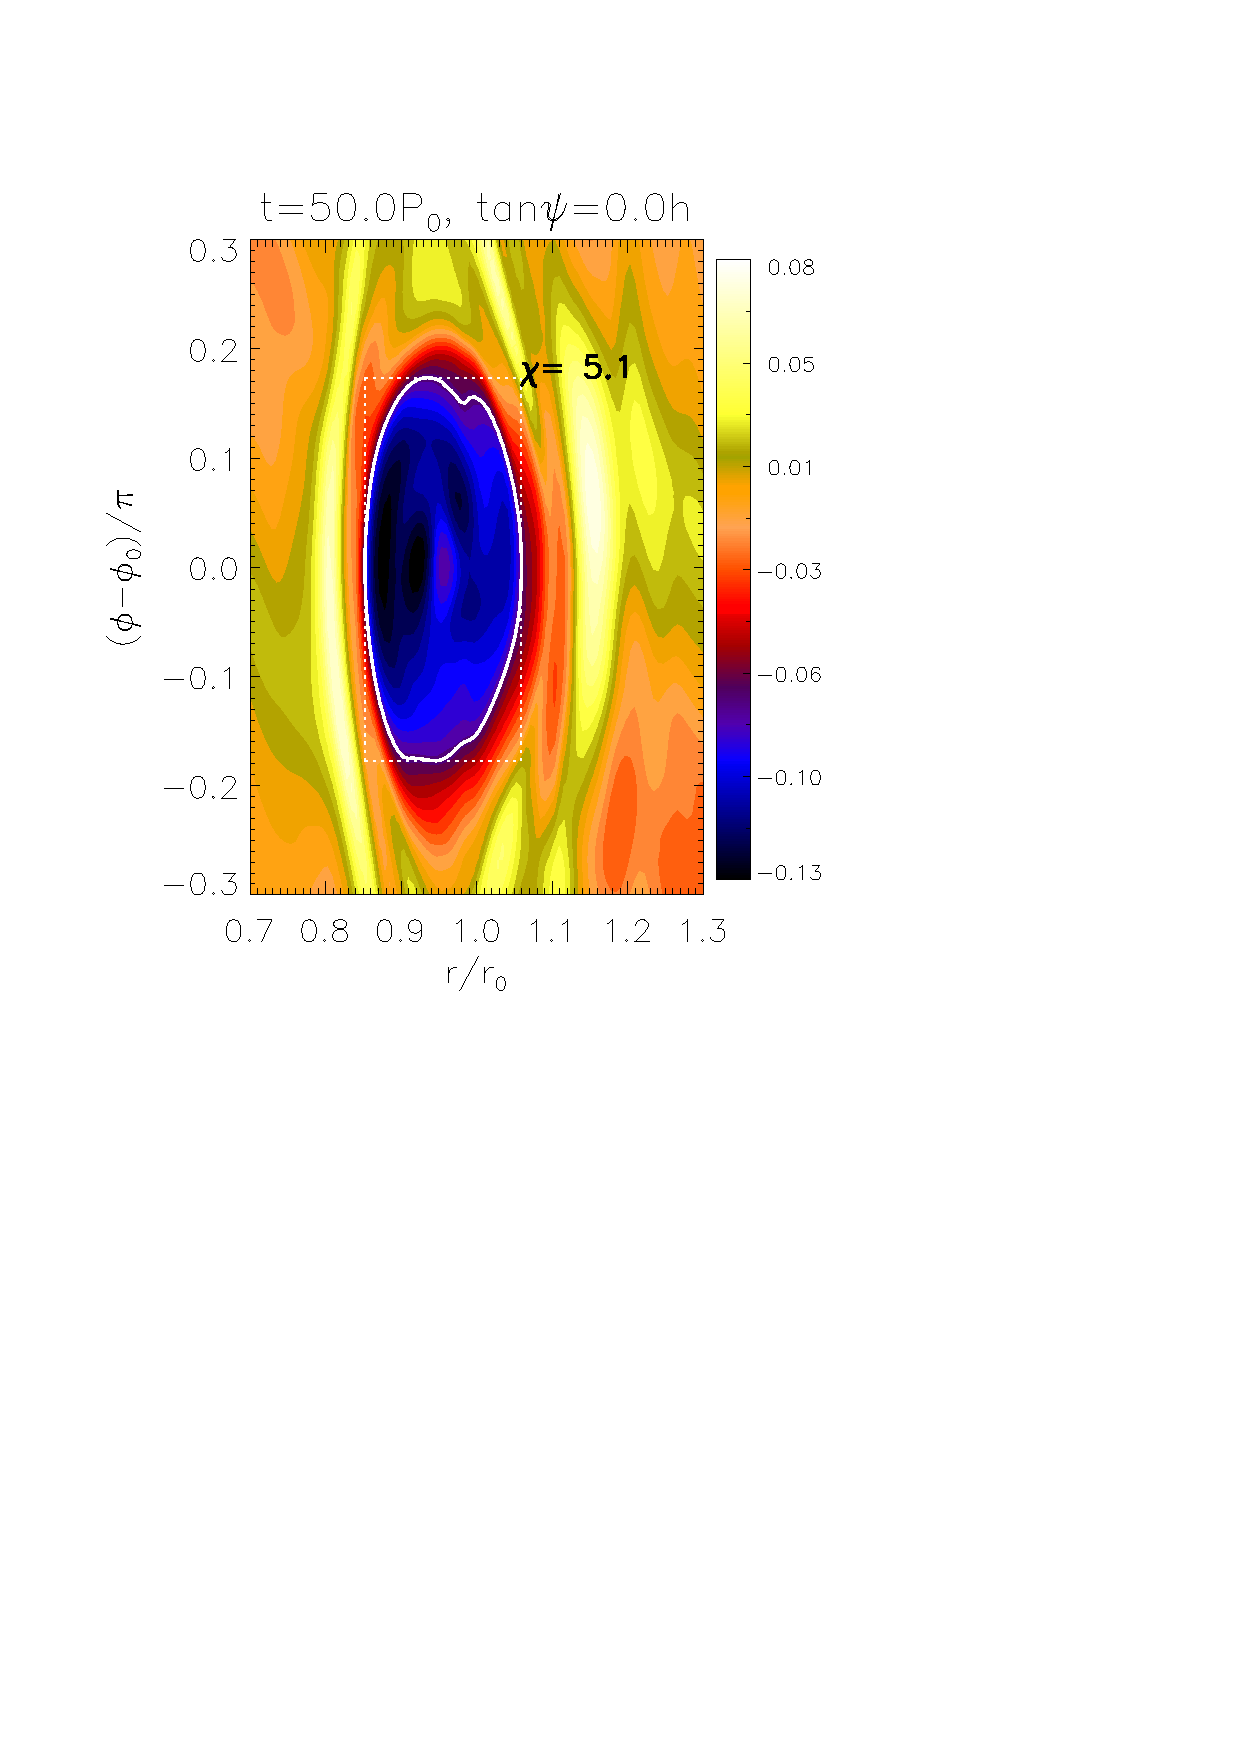
\includegraphics[scale=.27,clip=true,trim=2.3cm
     0.cm 0cm
     0cm]{figures/bump0_vort005}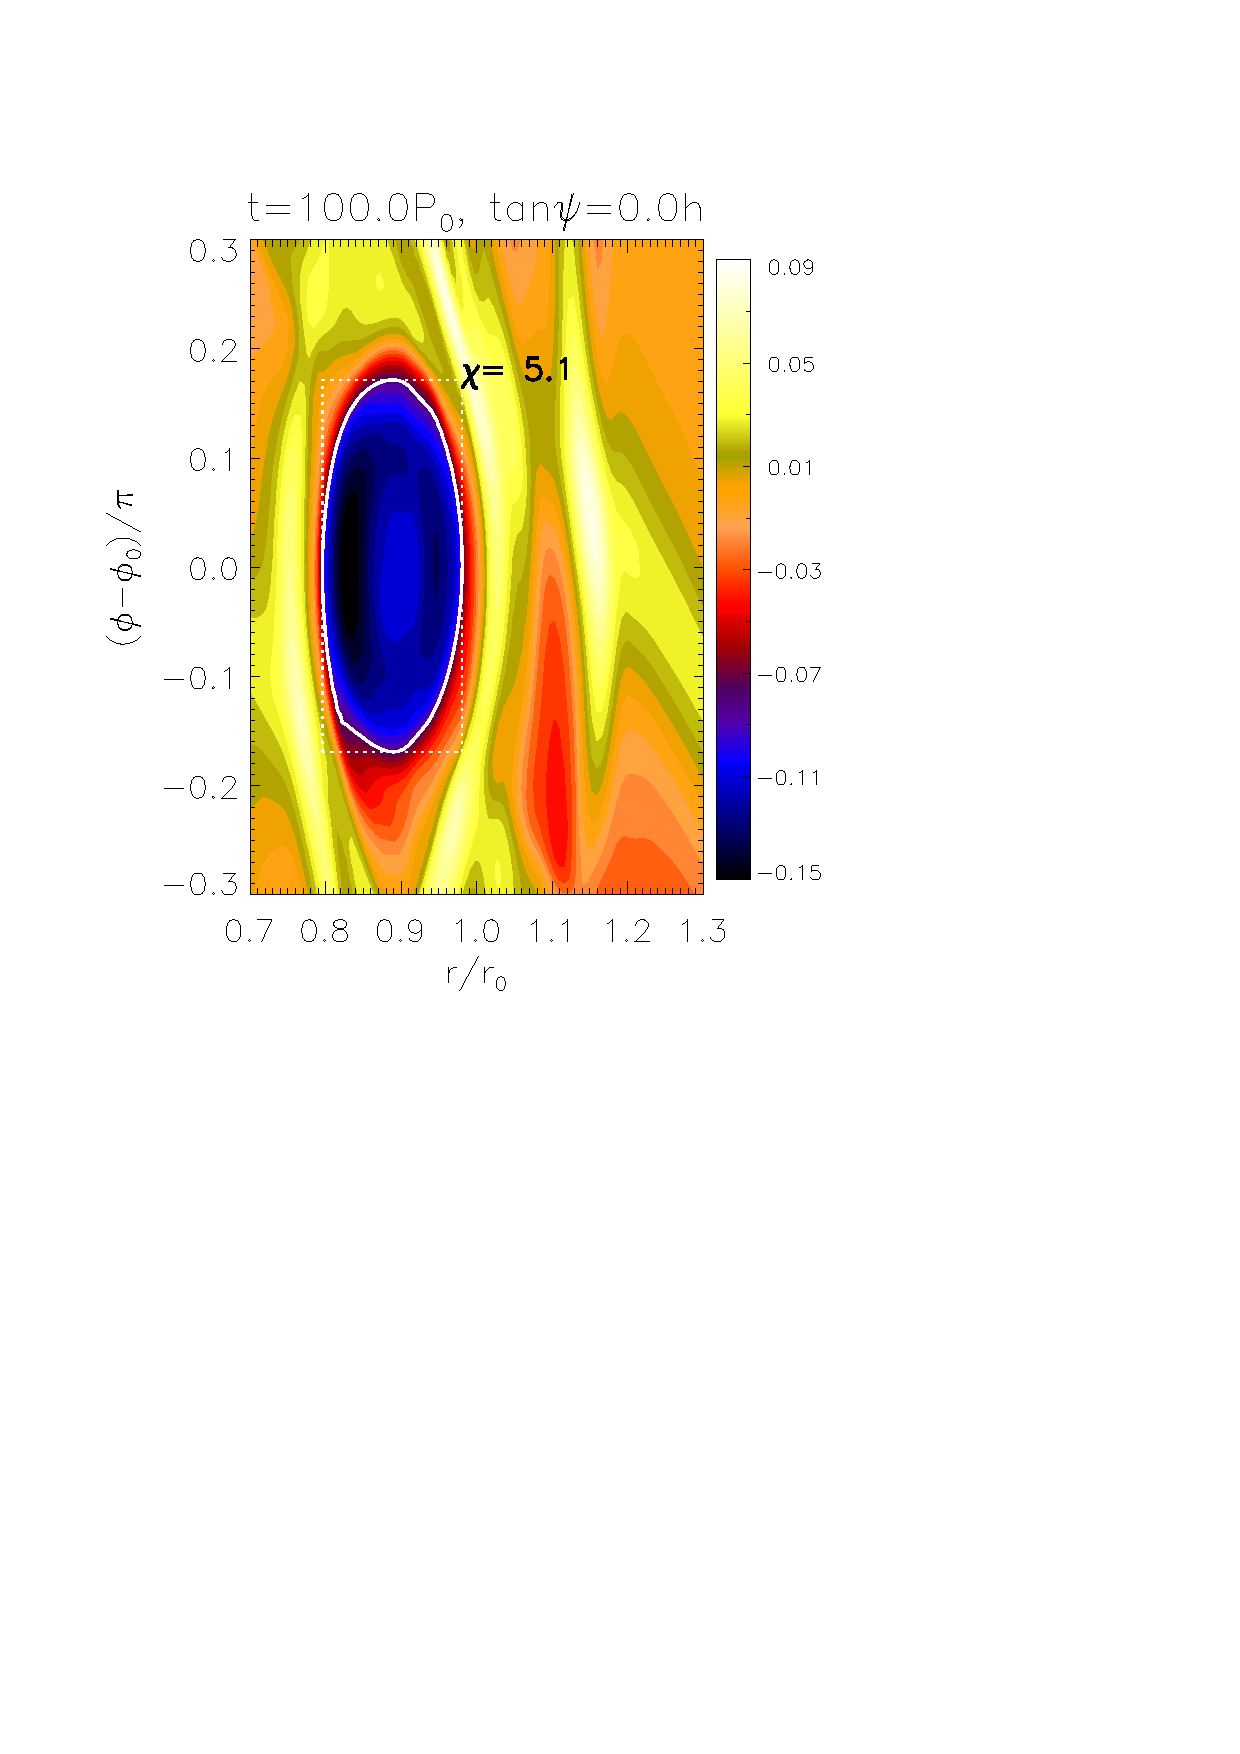
\includegraphics[scale=.27,clip=true,clip=true,trim=2.3cm
     0.cm 0cm
     0cm]{figures/bump0_vort010}
   \caption{Evolution of the midplane Rossby number, $Ro(z=0)$, for
     the inviscid case B0. $\chi$ is the
     width-to-length aspect ratio of the dotted boxes. 
     \label{bump0_bump1_vort}}
\end{figure}



\subsection{The effect of a viscous layer}
We now examine viscous cases V0 --- V3. Recall  
from Table \ref{artificial_bump} that the 
thickness of the upper viscous layer increases from case V0 to case
V3. At the reference radius, the viscous layer occupies
$0\%,\,25\%,\,50\%$ and $100\%$ of the vertical domain for cases V0, 
V1, V2 and V3, respectively.   

We first compare the control case V0 to the fiducial
inviscid case B0. Table \ref{artificial_bump} shows that despite
increasing the viscosity by a factor of $10^3$, the change to the
linear mode frequencies are negligible in going from case B0 to
V0. The value of $a_m$ and minimum Rossby number show that the final
vortex in V0 is only slightly weaker than that in B0. This is also
reflected in  Fig. \ref{bump0_bump1}---\ref{bump0_bump1_vort} (case B0) and the top panels of
Fig. \ref{vdamp0}---\ref{vdamp0_vort} (case V0), with a more elongated
vortex and smaller $|\Delta\rho|$ in V0 than in B0. 
%However, the vortex is more
%elongated in the non-linear regime (comparing the top panel of
%Fig. \ref{vdamp0_vort} to that of Fig. \ref{bump0_bump1}).  

As we increase the thickness of the viscous layer from case V0 to V3, 
Table \ref{artificial_bump} shows the dominant linear mode remains at
$m=4$, but linear growth rate does appreciably decrease 
(by $\sim 34\%$ from case V0 to V3). However, the linear growth timescales
are still $O(P_0)$.  
%It remains fast compared to the viscous time-scale
%associated with length-scales of order $H$. 
The effect of viscosity on the instability through the linear
perturbations is not significant as the RWI remains dynamical even in
the high-viscosity disc.   

%%%%%%%
Fig. \ref{vdamp0} show the density fluctuations of the
viscous cases. Comparing the second panel in Fig. \ref{vdamp0} (case
V1) to the top panel (case V0), we see that introducing the
viscous layer lengthens the lifetime of the density perturbation in the
nonlinear regime, since $\max(\Delta\rho)\simeq 0.47$ is maintained for
the second half of the simulation for case V1, but this value decreases
by about 0.1 for case V0 over the same timescale. 

Increasing the viscous layer further to case V2 and V3, we observe an
increase in the dominant azimuthal wavenumber in the nonlinear phase
(third and fourth panels in Fig. \ref{vdamp0}).  While
$\max(\Delta\rho)$ decreases with increasing viscosity, its
distribution becomes more global. %smaller density fluc. because  
%background viscosity is axisymmetric

\begin{figure}
   \centering
   \includegraphics[scale=.39,clip=true,trim=0cm 1.84cm 0cm
     0cm]{figures/vdamp0_pdisk005}\includegraphics[scale=.39,clip=true,trim=2.3cm
     1.84cm 0cm
     0cm]{figures/vdamp0_pdisk010}\\
    \includegraphics[scale=.39,clip=true,trim=0cm 1.84cm 0cm
     0.99cm]{figures/vdamp2_pdisk005}\includegraphics[scale=.39,clip=true,trim=2.3cm
     1.84cm 0cm
     0.99cm]{figures/vdamp2_pdisk010}\\
   \includegraphics[scale=.39,clip=true,trim=0cm 1.84cm 0cm
     0.99cm]{figures/vdamp3_pdisk005}\includegraphics[scale=.39,clip=true,trim=2.3cm
     1.84cm 0cm
     0.99cm]{figures/vdamp3_pdisk010}\\
   \includegraphics[scale=.39,clip=true,trim=0cm 0cm 0cm
     0.99cm]{figures/vdamp0_nu4_pdisk005}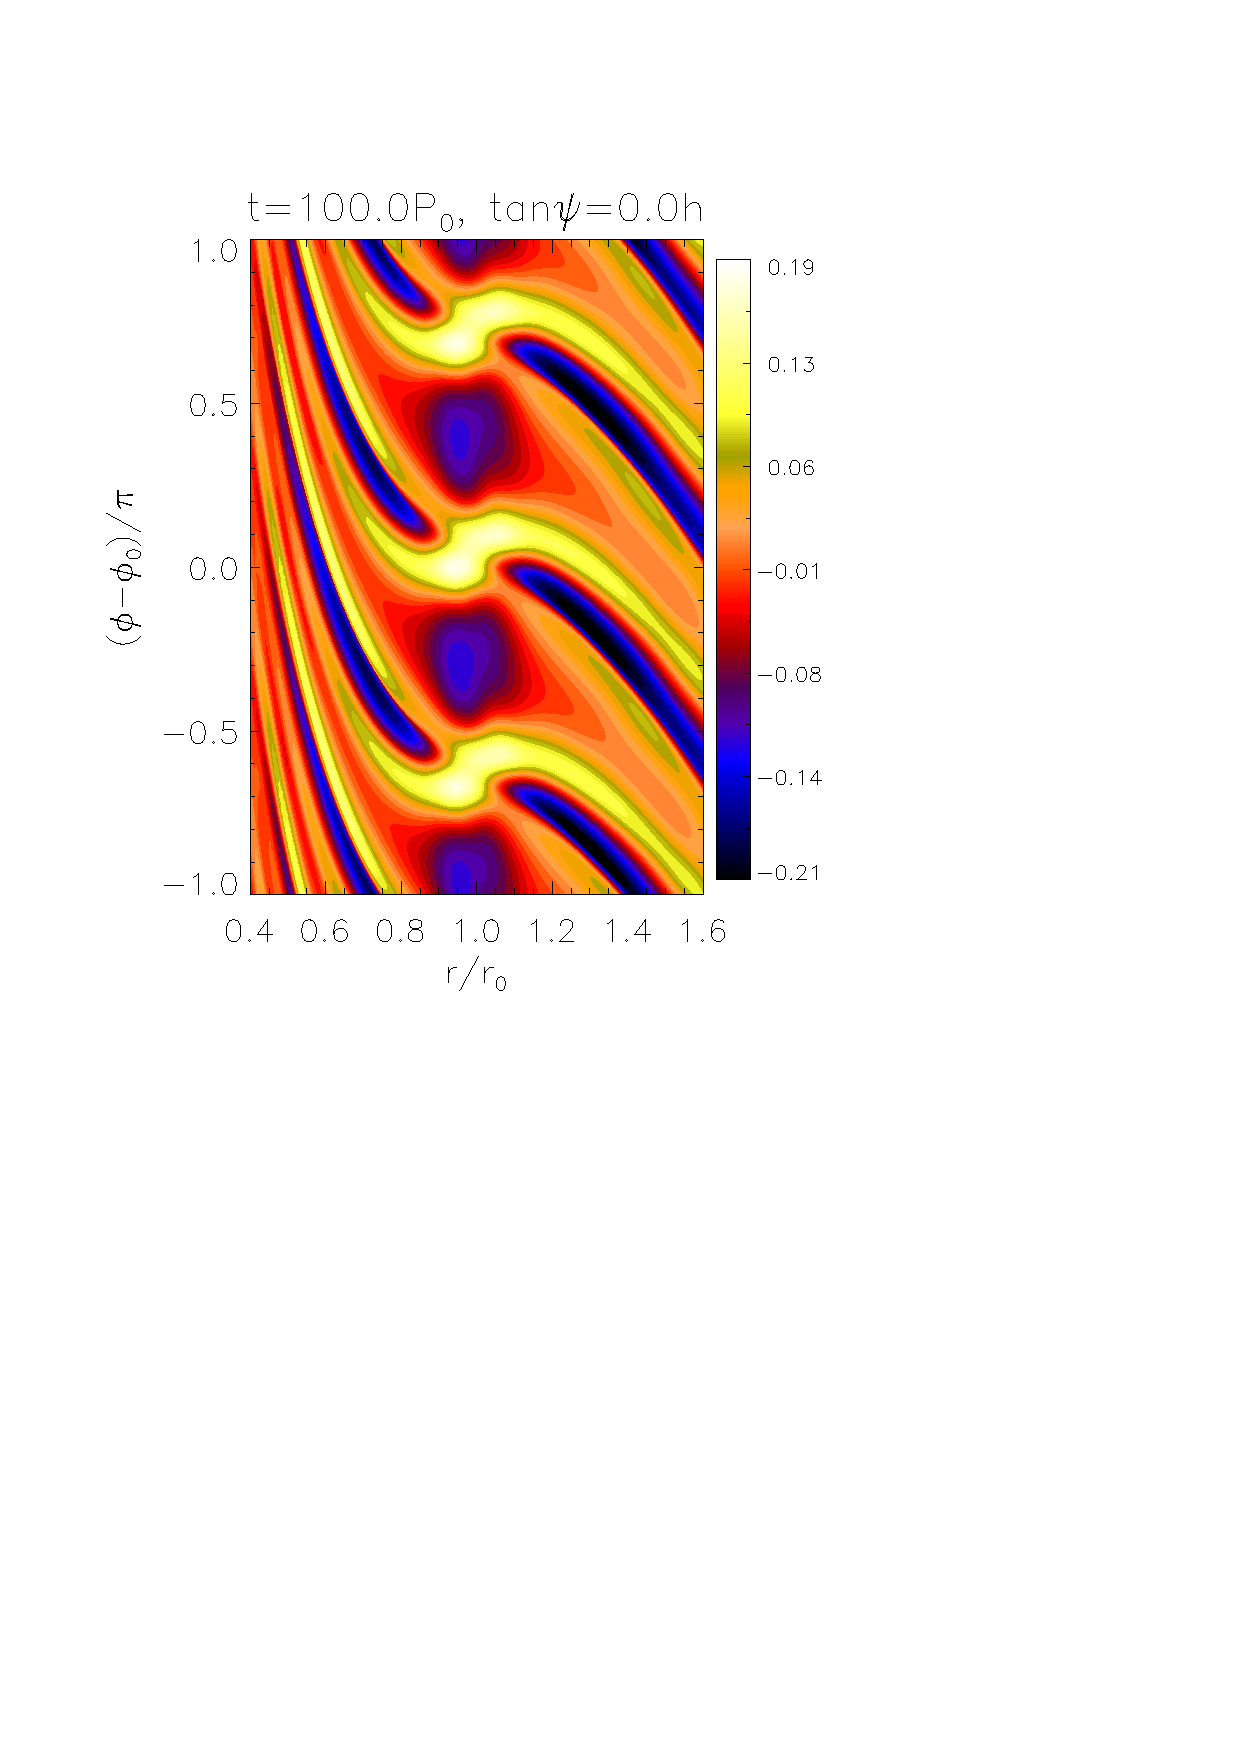
\includegraphics[scale=.39,clip=true,trim=2.3cm
   0.0cm 0cm
   0.99cm]{figures/vdamp0_nu4_pdisk010}
%%
   %% \includegraphics[scale=.42,clip=true,trim=0cm 1.84cm 0cm
   %%   0cm]{figures/vdamp0_pdisk005}\includegraphics[scale=.42,clip=true,trim=2.3cm 1.84cm 0cm
   %%   0.cm]{figures/vdamp2_pdisk005}\includegraphics[scale=.42,clip=true,trim=2.3cm 1.84cm 0cm
   %%   0.cm]{figures/vdamp3_pdisk005} \includegraphics[scale=.42,clip=true,trim=2.3cm 1.84cm 0cm
   %%   0.cm]{figures/vdamp0_nu4_pdisk005}\\
   %% \includegraphics[scale=.42,clip=true,trim=0.0cm
   %%   0.cm 0cm 0.cm]{figures/vdamp0_pdisk010}\includegraphics[scale=.42,clip=true,trim=2.3cm
   %%   0.cm 0cm 0.cm]{figures/vdamp2_pdisk010}\includegraphics[scale=.42,clip=true,trim=2.3cm
   %%   0.0cm 0cm 0.cm]{figures/vdamp3_pdisk010}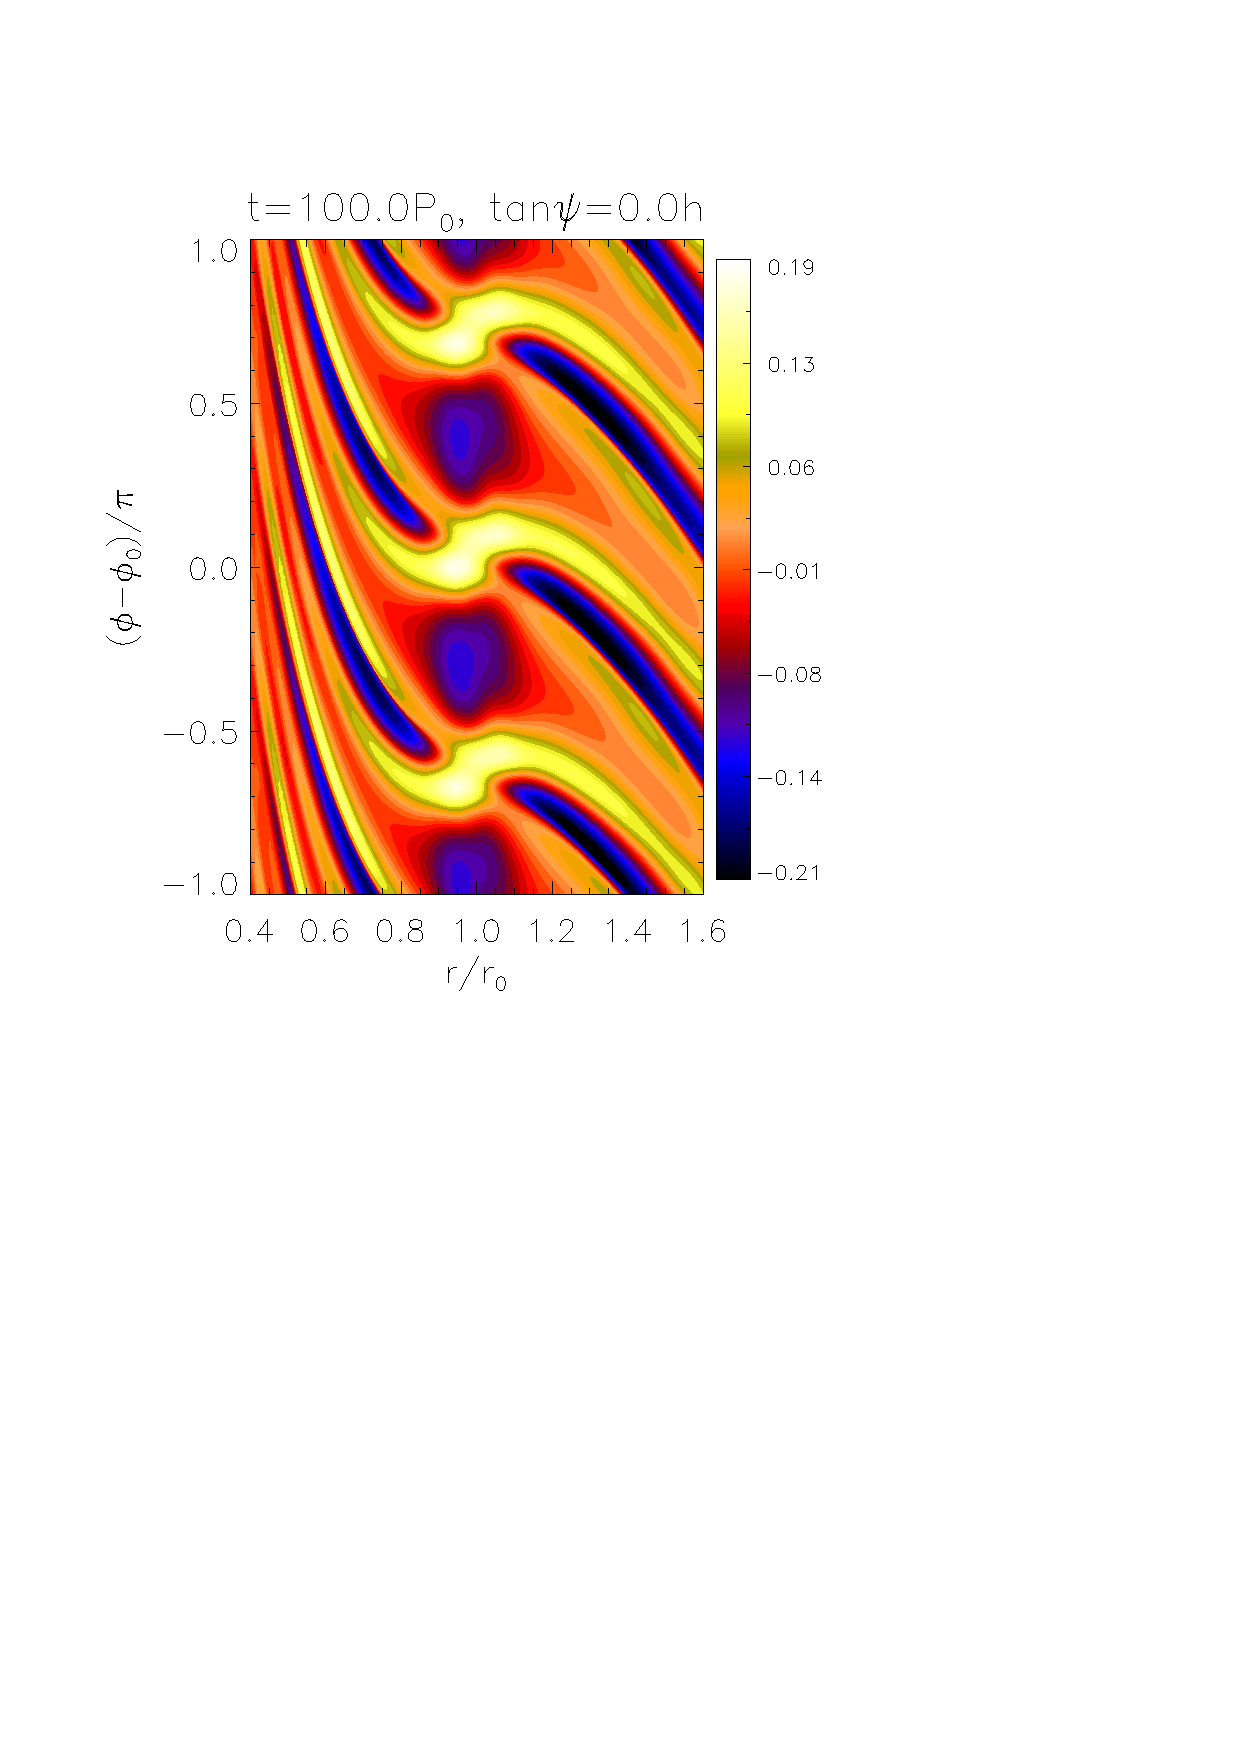
\includegraphics[scale=.42,clip=true,trim=2.3cm
   %%   0.0cm 0cm 0.cm]{figures/vdamp0_nu4_pdisk010}
   \caption{Non-axisymemtric density field at the midplane
     $\Delta\rho(z=0)$ for viscous cases V0, V1, V2 and V3 (top to
     bottom). $\phi_0$ is the azimuth of $\max[\Delta\rho(z=0)]$. 
     \label{vdamp0}}
\end{figure}

Fig. \ref{vdamp0_vort} compares the Rossby number associated with the
over-densities produced by the RWI. Thickening the viscous 
layer decreases the vortex aspect-ratio. Since their widths remain
at $\sim 2H_0$, the vortices become smaller with increasing
viscosity. This may be partly attributed to fewer vortex merging
events having occured as viscosity is increased. The merging of
two vortices usually leads to a larger but weaker vortex (smaller
$|Ro|$), so if vortex merging is resisted then each vortex may evolve
separately. Vortices then become stronger as viscosity is increased
(more negative $Ro$).

\begin{figure}
   \centering
   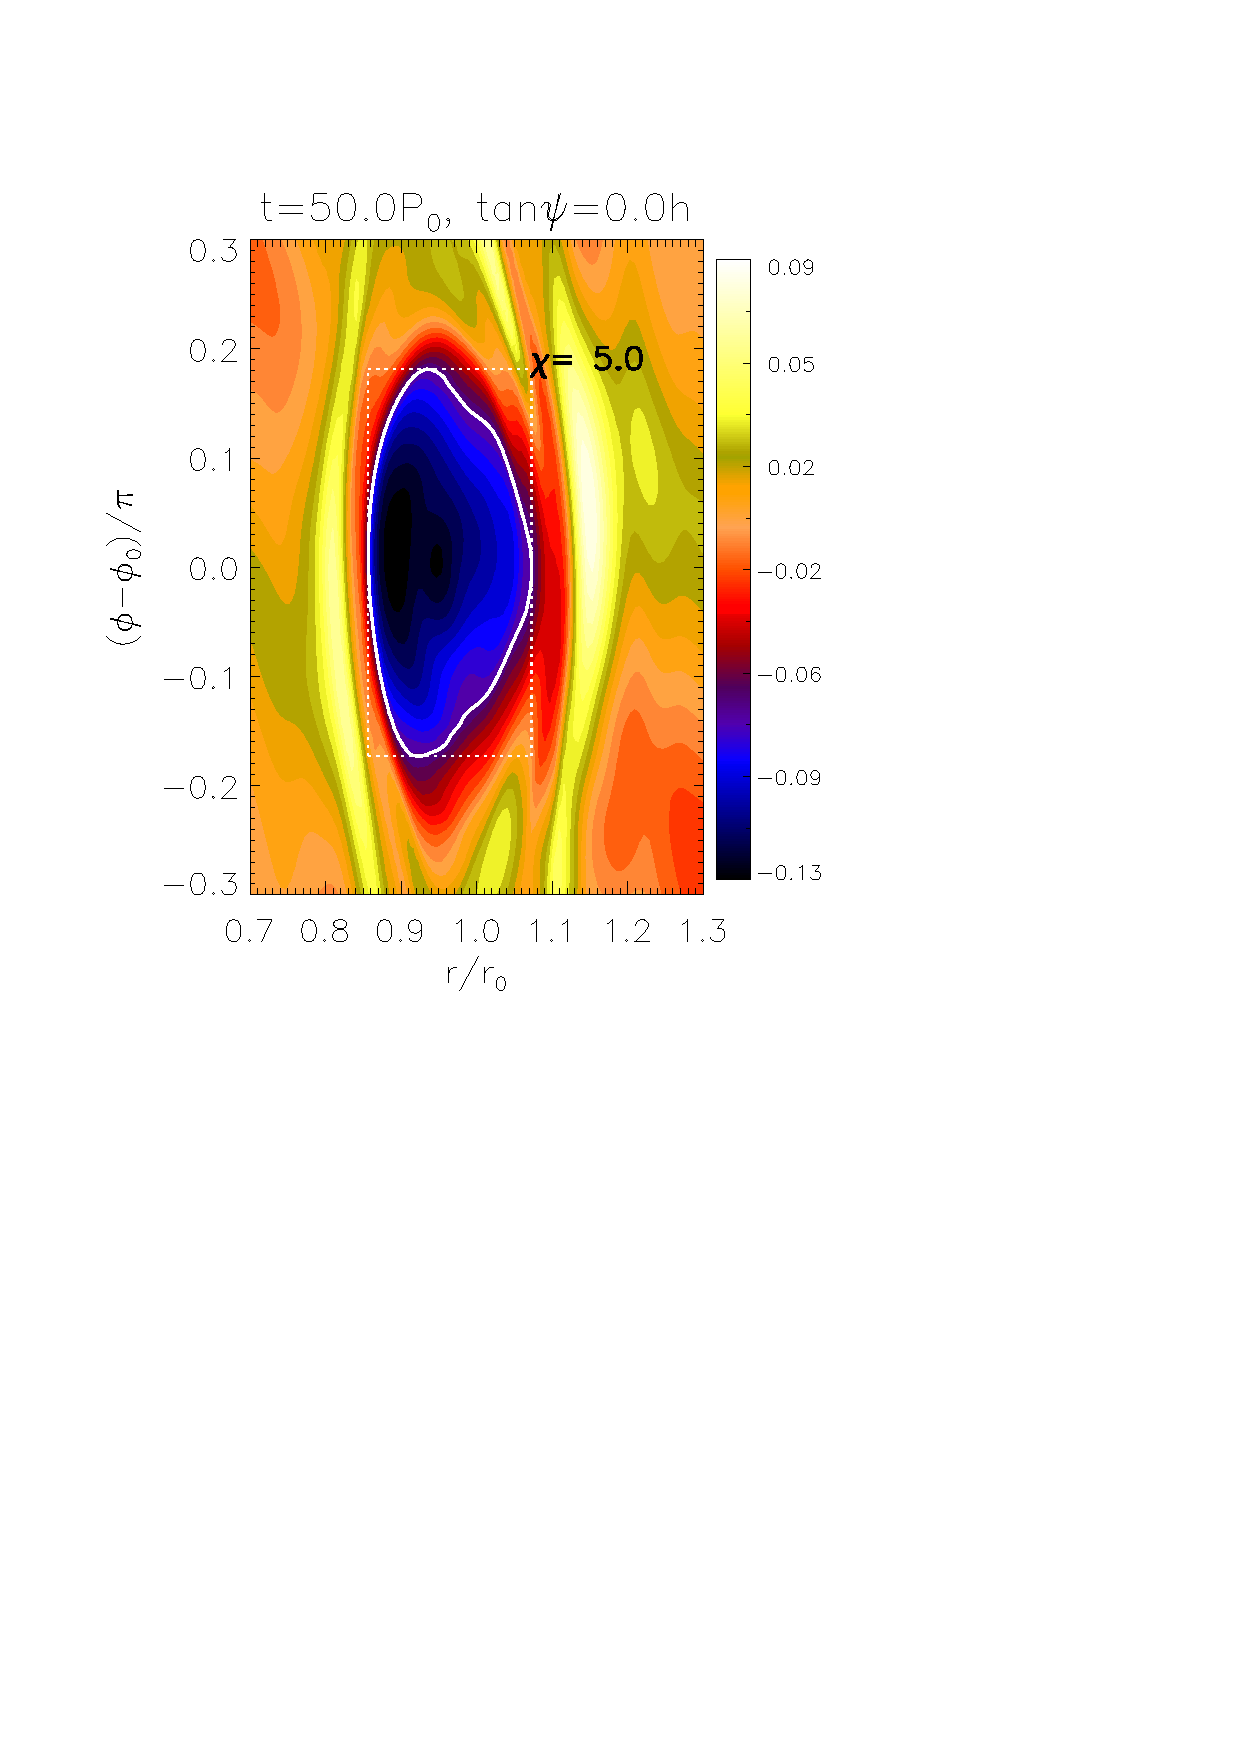
\includegraphics[scale=.39,clip=true,trim=0cm 1.84cm 0cm
     0cm]{figures/vdamp0_vort005}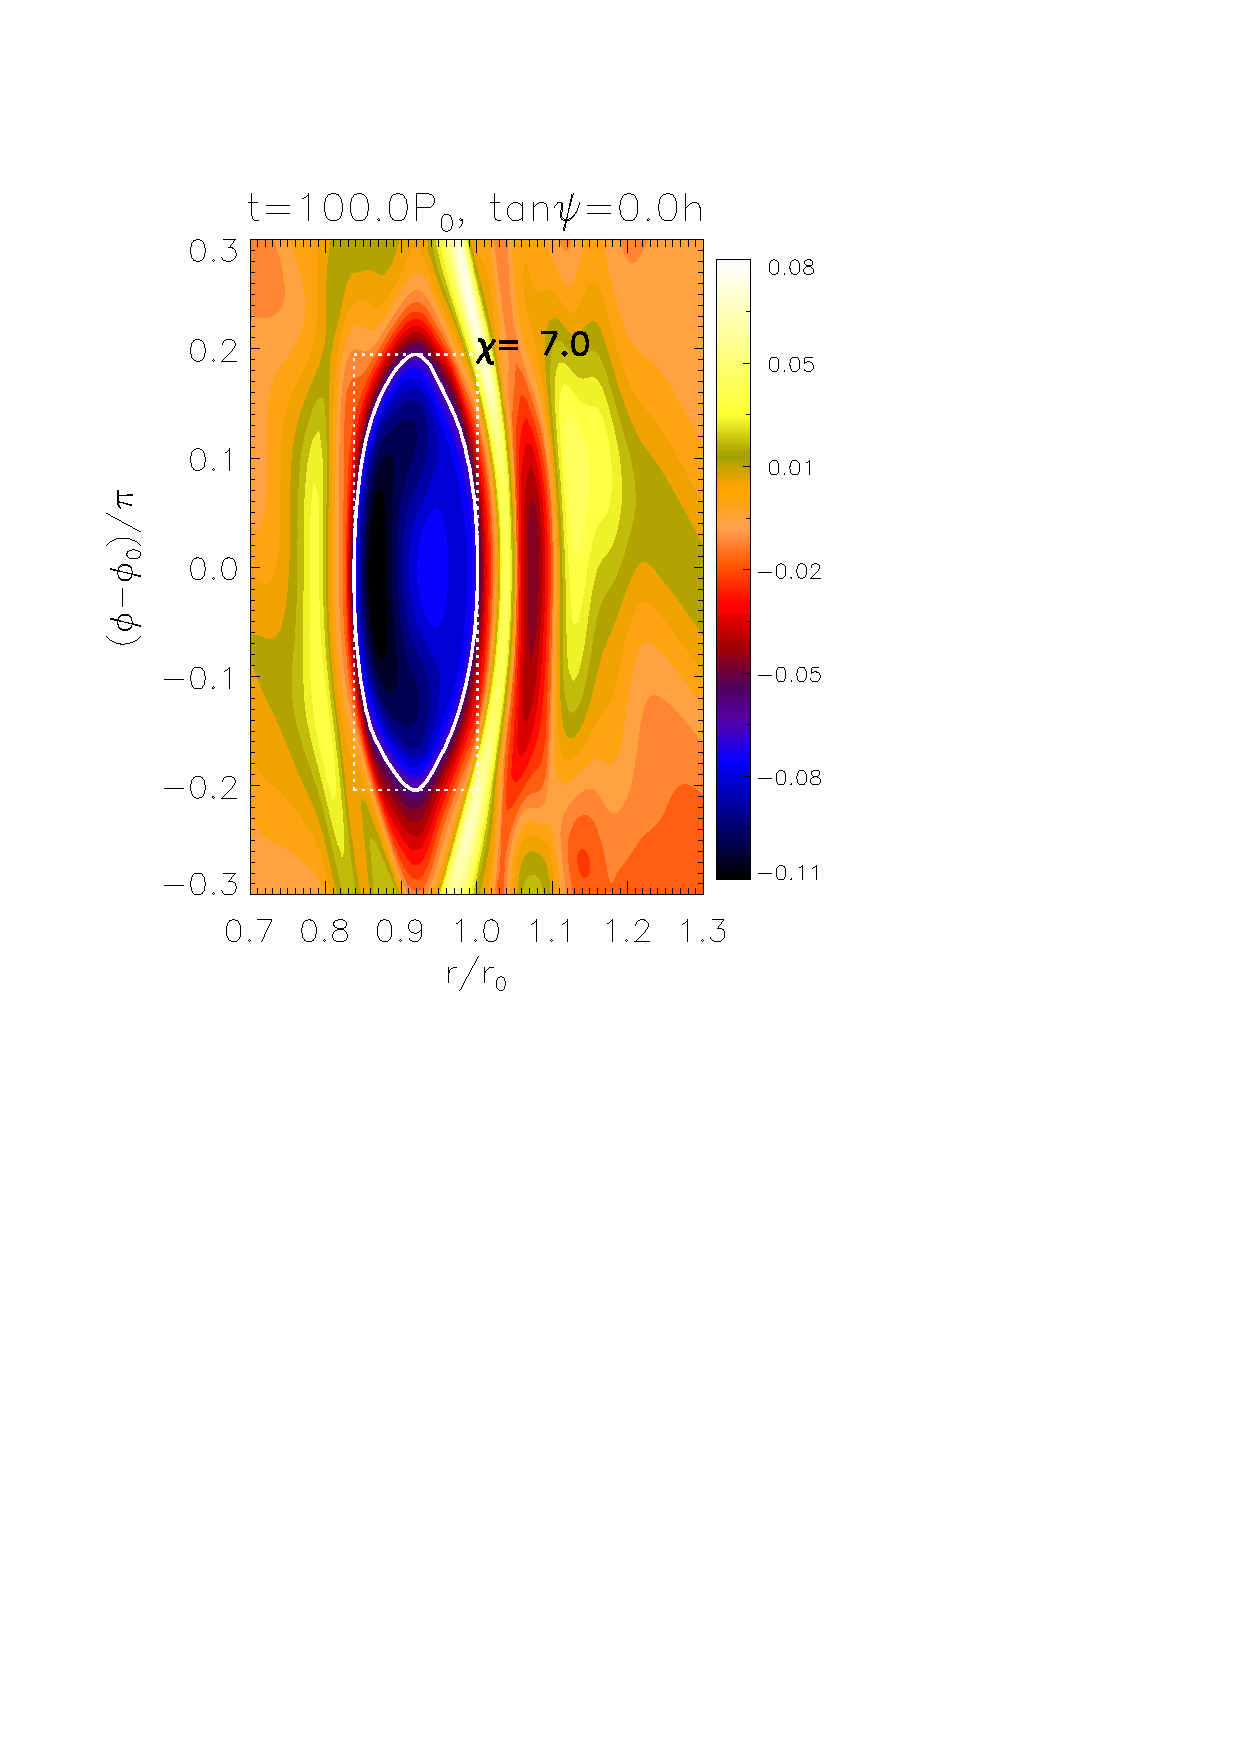
\includegraphics[scale=.39,clip=true,trim=2.3cm
     1.84cm 0cm
     0cm]{figures/vdamp0_vort010}\\
   \includegraphics[scale=.39,clip=true,trim=0cm 1.84cm 0cm
     0.99cm]{figures/vdamp2_vort005}\includegraphics[scale=.39,clip=true,trim=2.3cm
     1.84cm 0cm
     0.99cm]{figures/vdamp2_vort010}\\
   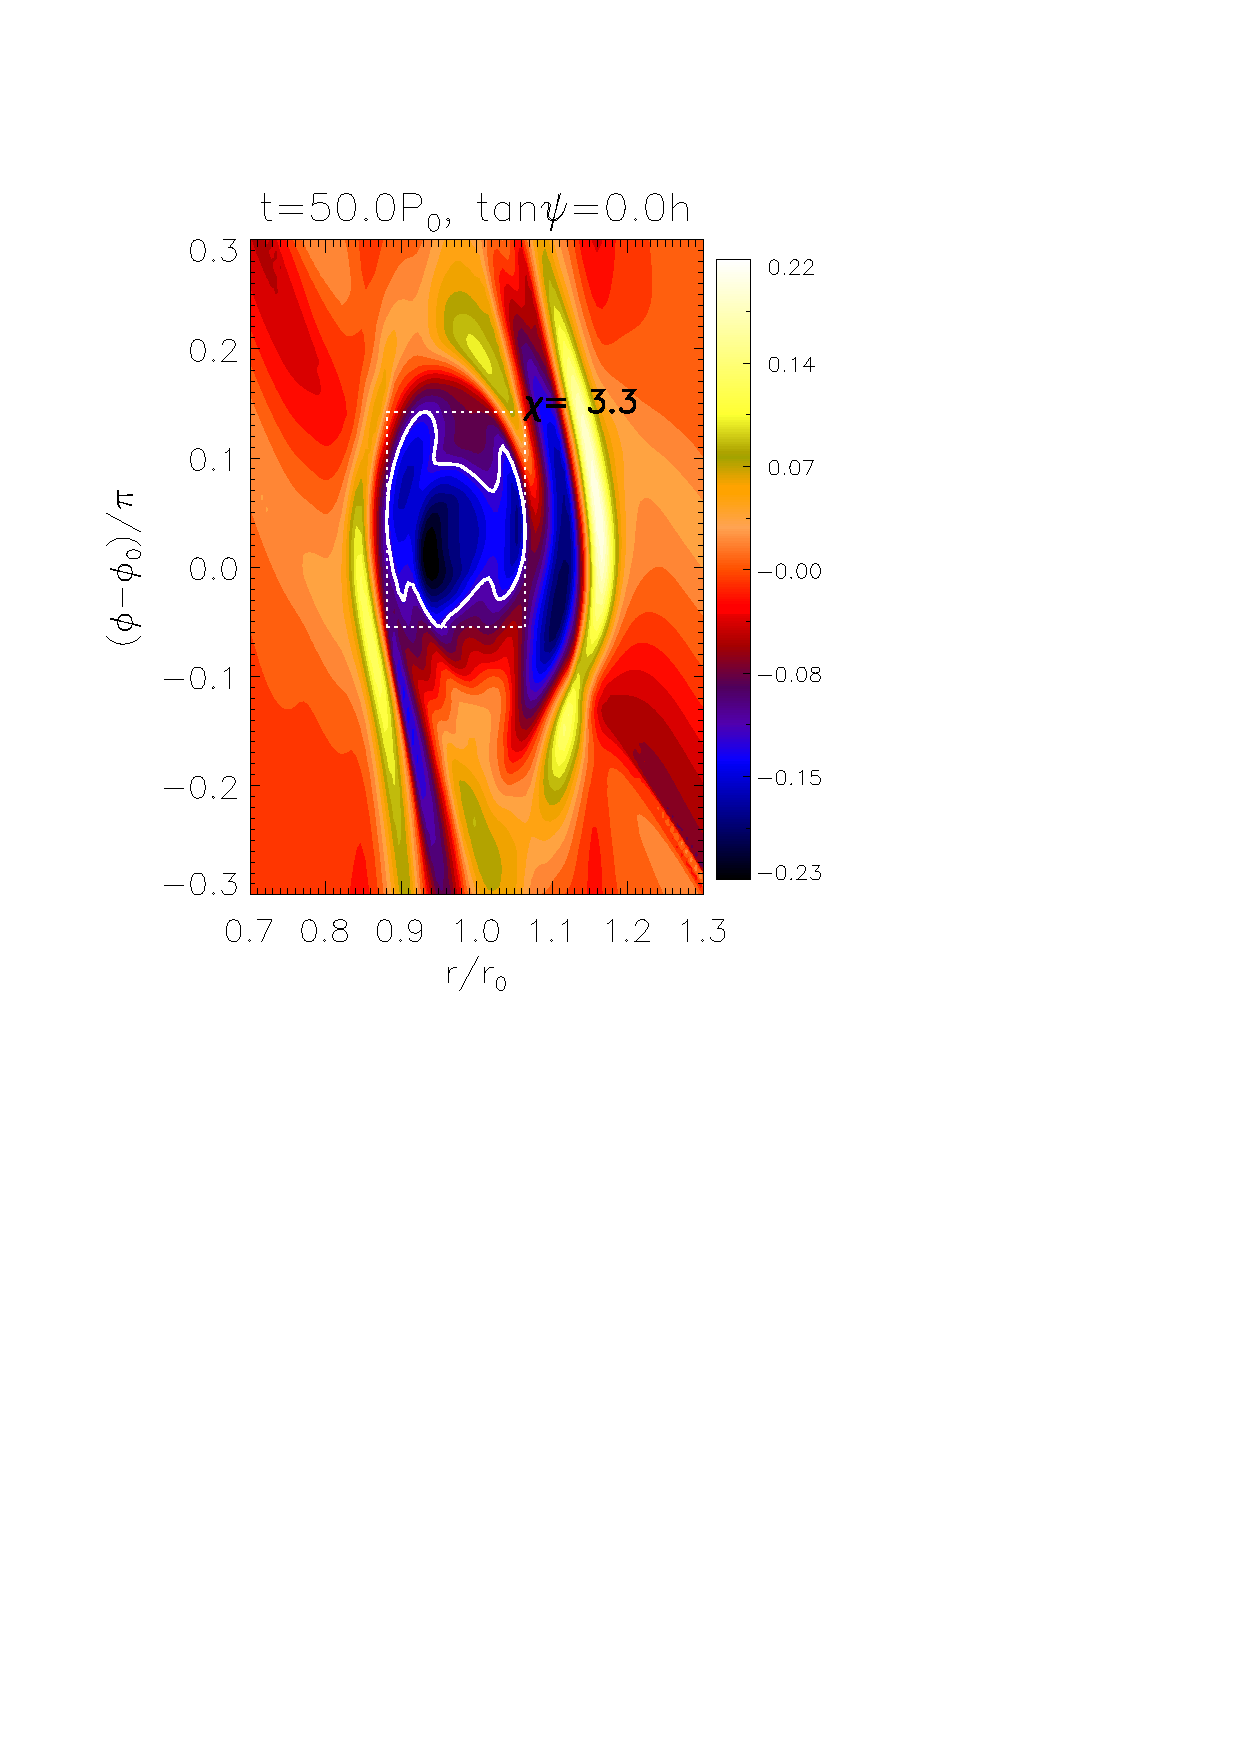
\includegraphics[scale=.39,clip=true,trim=0cm 1.84cm 0cm
     0.99cm]{figures/vdamp3_vort005}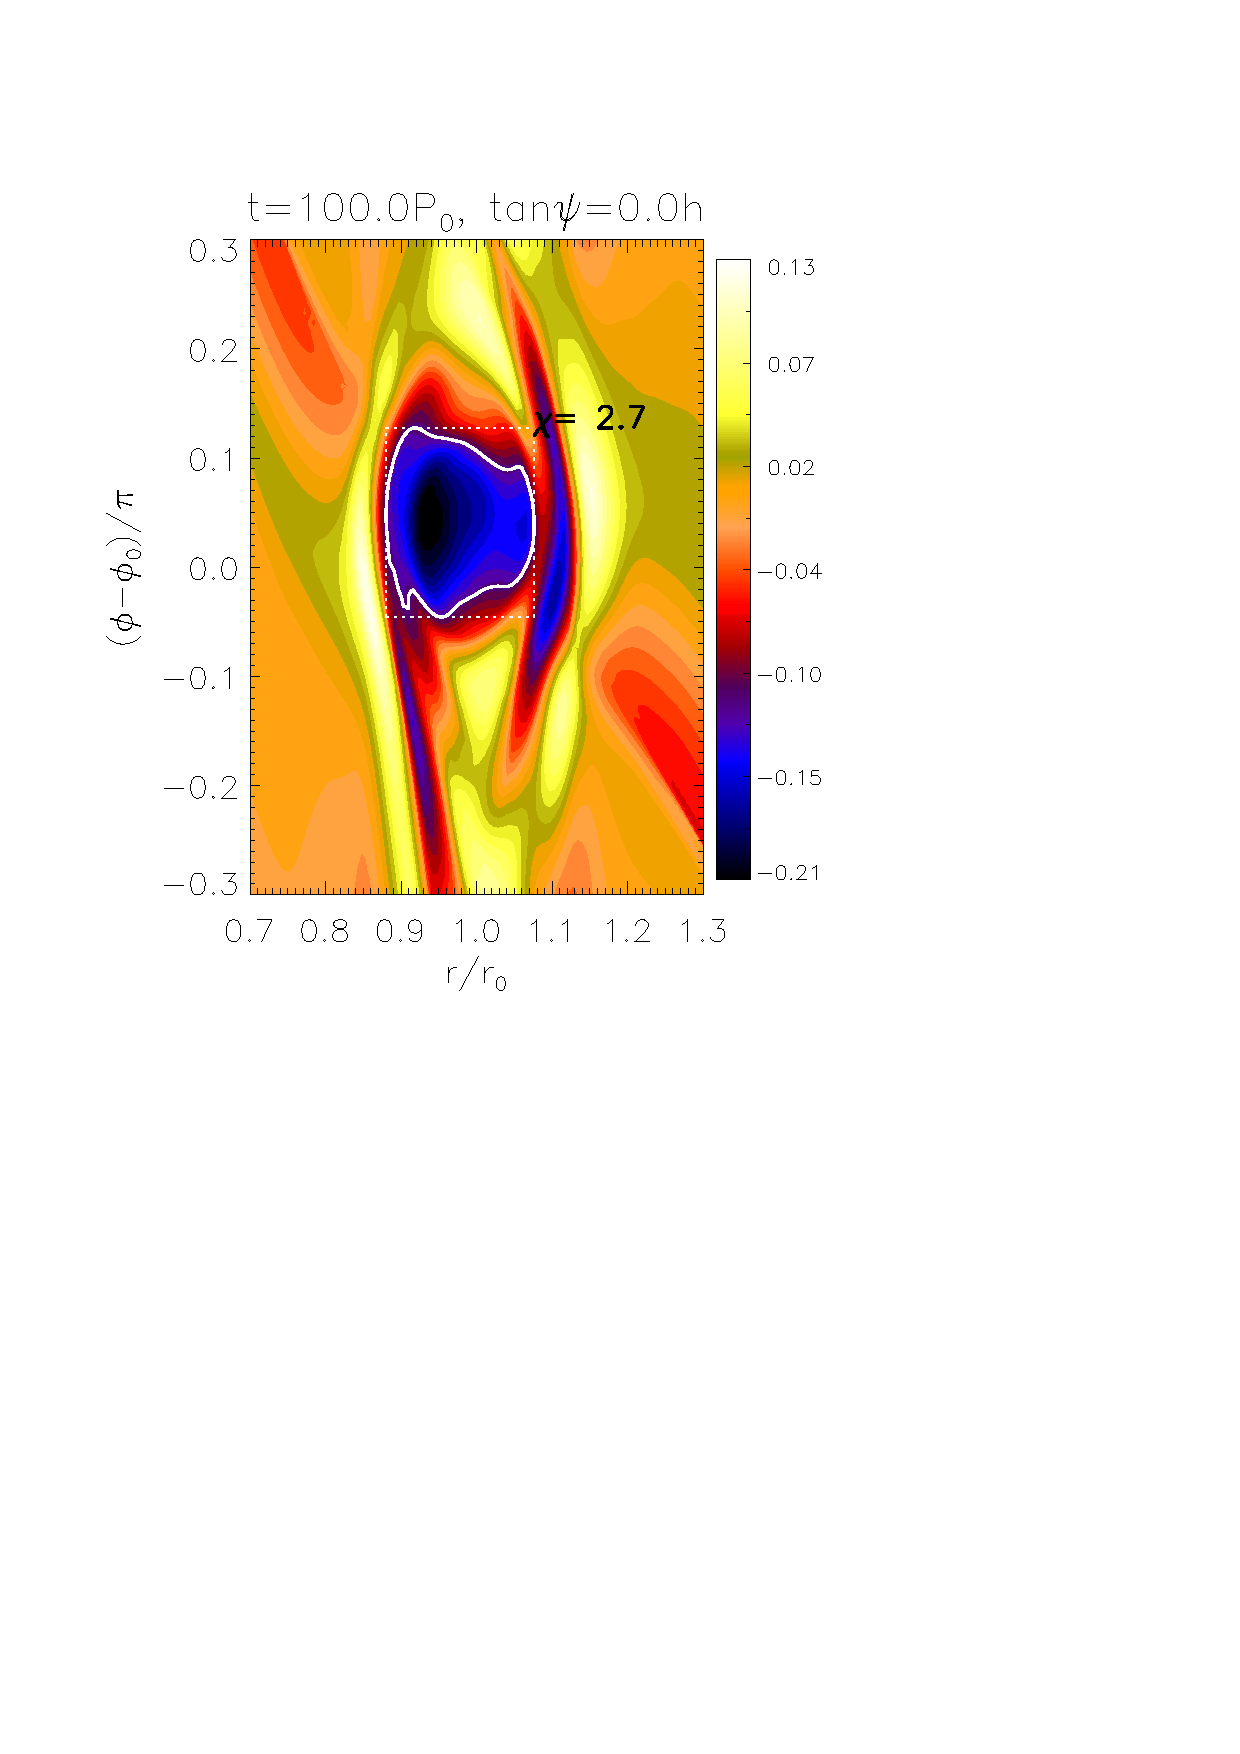
\includegraphics[scale=.39,clip=true,trim=2.3cm
     1.84cm 0cm
     0.99cm]{figures/vdamp3_vort010} \\
   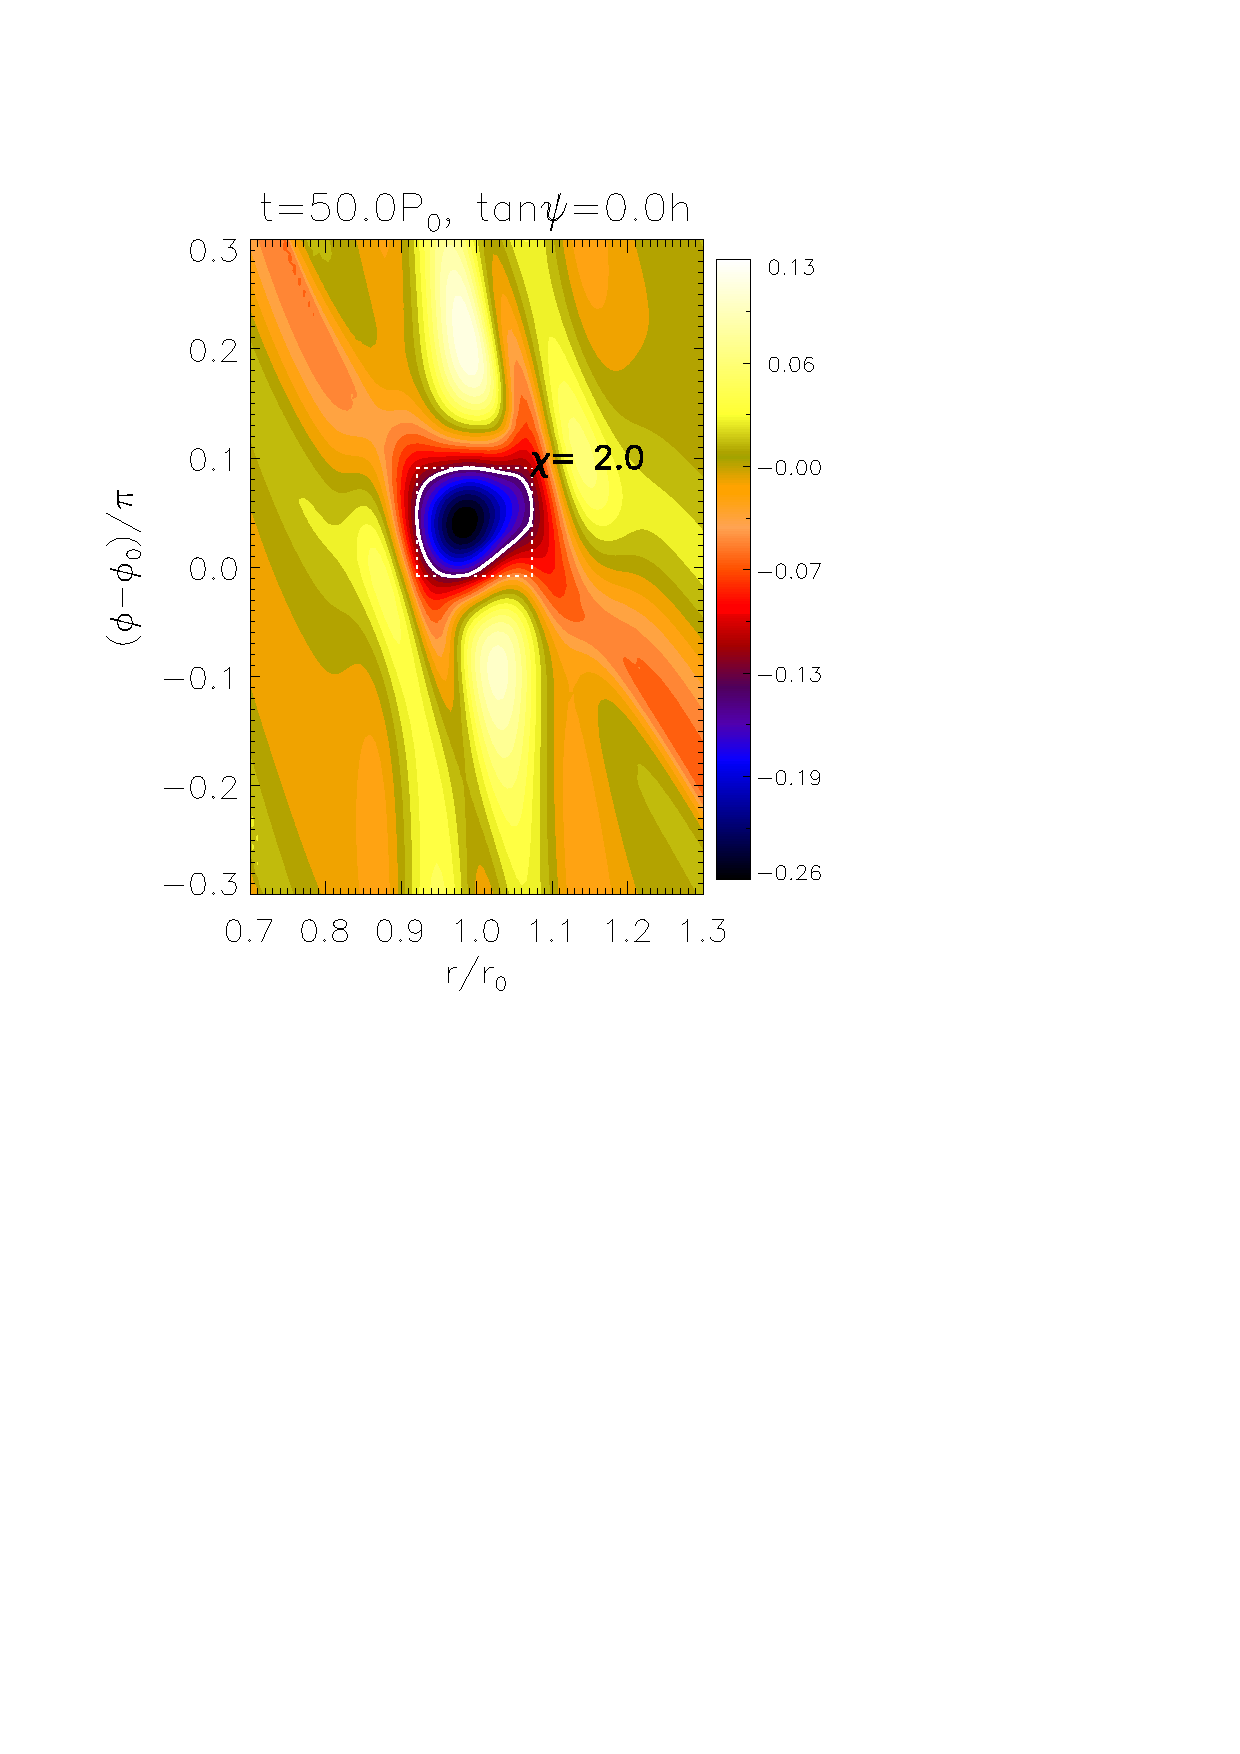
\includegraphics[scale=.39,clip=true,trim=0cm 0cm 0cm
     0.99cm]{figures/vdamp0_nu4_vort005}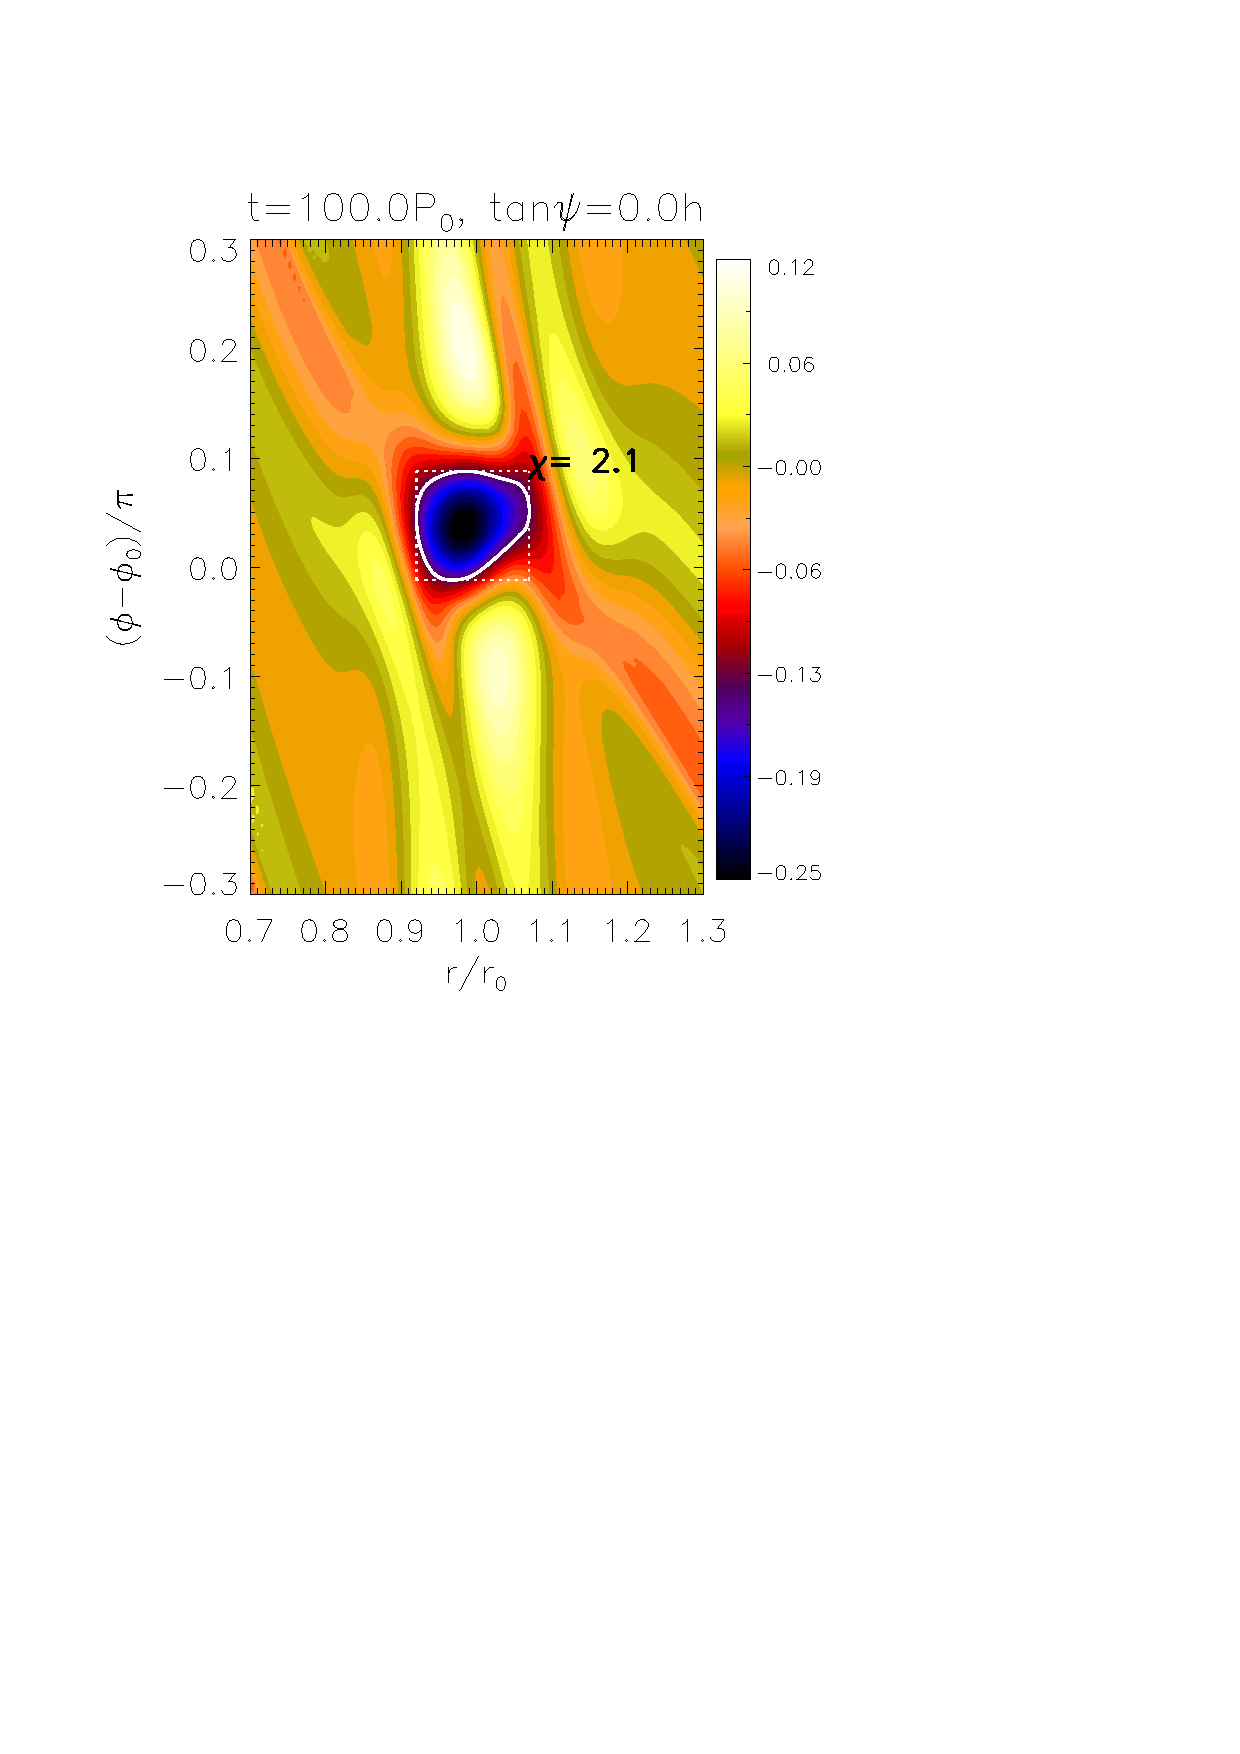
\includegraphics[scale=.39,clip=true,trim=2.3cm
     0.0cm 0cm
     0.99cm]{figures/vdamp0_nu4_vort010}
   \caption{Midplane Rossby number
     $Ro(z=0)$ for viscous cases V0, V1, V2 and V3 (top to
     bottom). 
     \label{vdamp0_vort}}
\end{figure}

Notice the difference between the snapshots taken at $t=50P_0$ and at
$t=100P_0$ in Fig. \ref{vdamp0}---\ref{vdamp0_vort}
diminishes with increasing viscosity. In fact, we found the
high-viscosity case V3 reached steady-state after $t\geq40P_0$. Thus,
with increasing viscosity the system resists nonlinear vortex merging
%evolution is halted  
to produce a single vortex, which usually occurs on a dynamical
timescale in inviscid simulations (case B0). 

%%%%%%%%%%%%%%%%%%%%%%%%%%%%%%%%%%%%%%%%%%%%%%%%%%%%%%%%%%%%%%%%%%%%


\subsubsection{Order of magnitude comparison of timescales}
The observation of stronger vortical structures (more negative $Ro$
and smaller vortex aspect-ratio) with increasing
viscosity is unexpected, since one normally expects viscosity to
smooth out the flow. We can make sense of this result by comparing key
timescales relevant to the problem. 

The characteristic spatial scale of the background density bump and of
the instability is the local scale-height $H$, so the associated
viscous timescale is    
\begin{align}
  t_\nu = \frac{H^2}{\nu}\sim \frac{h^2}{\hat{\nu}\Omega}. 
\end{align}
The linear instability growth timescale is
\begin{align}
  t_\mathrm{RWI} = \frac{1}{\epsilon \Omega},
\end{align}
where $\epsilon$ is found from numerical simulations. 
The ratio of these timescales is
\begin{align}
  \frac{t_\nu}{t_\mathrm{RWI}} \sim \frac{\epsilon h^2}{\hat{\nu}}.
\end{align}
Table \ref{artificial_bump} indicates $\epsilon \sim 0.1$. 
Inserting $h=0.1$ and $\hat{\nu}=10^{-4}$ gives $t_\nu \sim 10
t_\mathrm{RWI}$. That is, viscosity damping is slower than linear
growth, even for the highest viscosity values we consider. The linear
phase of the instability is therefore unaffected by viscosity. 

\cite{meheut13} argued that $t_\mathrm{RWI}$ is also the vortex
turn-over time $t_\mathrm{turn}$ when the instability saturates and
the linear phase terminates. Then 
$t_\nu\sim 10 t_\mathrm{turn}$, implying viscous effects 
are unimportant over a turn-over time. 
However, if we estimate a vortex turn-over time as $t_\mathrm{turn}
\sim 2\pi/|Ro|\Omega$ then $t_\nu\sim (h^2|Ro|/2\pi\hat{\nu})t_\mathrm{turn}$.  
Inserting $h=0.1,\,\hat{\nu}=10^{-4}$ and $|Ro|=0.25$ (case V3) gives 
$t_\nu \sim 4t_\mathrm{turn}$. Therefore, depending on the vortex shape, 
$t_\nu$ may not be much larger than $t_\mathrm{turn}$. 

%% \cite[The inequality accounts for the fact that the
%% turn-over time is longer for more elogated vortices,][]{lesur09}. 
%Similarity between $t_\nu$ and $t_\mathrm{turn}$ suggest viscosity
%should have smoothed out the vortical structure. 

In any case, our simulations span several local viscous time-scales,
$t_\mathrm{sim}\sim 10t_\nu $, so viscous damping should
have taken place. On the contrary, $Ro$ becomes more negative as the
viscous layer increases from case V0 to V3. To rationalise this
observation, we recall that the RWI is fundamentally
associated with a vortensity minimum and the instability is stronger
for deeper minima \citep{li00}.  
%and the viscosity profile has been specially chosen to
%maintain such a structure in a steady state in the absence of
%perturbations.  

Consider the potential vorticity perturbation at the bump radius, which was
found to be  
\begin{align}\label{vortensity_pert}
  \left.\frac{\aziavg{\eta_z}(t=100P_0)}{\eta_z(t=0)}\right|_{R=r_0} - 1 = 
  \begin{cases}
    3.99  & \text{Case V0} \\
   3.03  & \text{Case V1} \\
   2.24  & \text{Case V2} \\
   1.71  & \text{Case V3} \\
  \end{cases}.
\end{align} 
(This value is 4.92 for the inviscid case B0.) The PV
perturbation is positive, so the initial PV minimum is weakened
by the vortices \citep{meheut10}. This effect
diminishes with increasing viscosity. One contributing factor is 
that viscosity reduces the linear growth rate, implying the linear
perturbations saturate at a smaller amplitude \citep{meheut13}. This
is expected to weaken the background axisymmetric structure to a lesser
extent.    

We also recall that in the present simulations, the time-independent
viscosity profile was specially chosen to be consistent with a
steady-state disc containing a localised PV minimum.  
That is, the viscosity profile is also radially structured. We suggest
that for such setups, viscosity attempts to restore the initial disc
profile, i.e. the initial PV minimum.   

When viscosity is small, the viscous timescale is long compared to our
simulation timescale. In this case the nonlinear evolution of the
instability---vortex formation---weakens the PV minimum with viscosity
playing no role. As we increase viscosity, the viscous timecale
associated with the density bump becomes shorter than our simulation
timescale. %deviations away from the initial bump is smoothed out by
            %viscosity 
This means that over the course of the simulation, our spatially-fixed
viscosity profile acts as a source of PV minimum. 

In essence, in the nonlinear regime there is competition
between destruction of the background PV minimum by the
vortices and reformation of the initial radial PV minimum by the
imposed viscosity profile. We except this latter to support the
instability, leading to stronger vortices.  

 
We point out that the snapshots in
Fig. \ref{vdamp0}---\ref{vdamp0_vort} are taken at the midplane, but  
the influence of viscosity is apparent even when comparing case V1 to
V0, i.e. when the viscous layer is confined near the upper
boundary. This demonstrates the vertically-global nature of vortex
formation through the RWI. Conditions near the disc
surface should be expected to influence the instability throughout the
fluid column. 



